\chapter{Последовательности и прогрессии}\markright{Глава 12}
\begin{definition}
\term{Числовая последовательность} (real sequence) — отображение \(a:\mathbb N\to\mathbb R\), где \(\mathbb N=\{1,2,3,\ldots\}\). Числу \(n\) соответствует \term{член последовательности} (term) \(a_n\); \(n\) — его номер. Последовательность записывают как \((a_n)_{n\geq1}\).
\end{definition}
\begin{definition}
\term{Формула общего члена} (explicit formula) непосредственно выражает \(a_n\) через \(n\). \term{Рекуррентная, или индуктивная, запись} (recursive definition) задаёт начальное значение и правило получения следующих членов из предыдущих. Например, \(a_1=2\), \(a_{n+1}=a_n+3\) при \(n\geq1\).
\end{definition}
\begin{definition}
\term{Арифметическая прогрессия} (arithmetic progression) — последовательность, для которой \(a_{n+1}=a_n+d\) при всех \(n\geq1\). Постоянное число \(d\) называют \term{разностью прогрессии} (common difference).
\end{definition}
\begin{theorem}[Общий член арифметической прогрессии]
Для арифметической прогрессии
\[
a_n=a_1+(n-1)d,\qquad n\geq1.
\]
\end{theorem}
\begin{proof}
При \(n=1\) равенство верно. Если \(a_k=a_1+(k-1)d\), то \(a_{k+1}=a_k+d=a_1+kd\). По математической индукции формула верна для всех \(n\geq1\).
\end{proof}
\begin{definition}
\term{Частичная сумма} (partial sum) последовательности — сумма первых \(N\) членов: \(S_N=a_1+\cdots+a_N\).
\end{definition}
\begin{theorem}[Сумма арифметической прогрессии]
\[
S_N=\frac{N(a_1+a_N)}{2}=\frac N2\bigl(2a_1+(N-1)d\bigr).
\]
\end{theorem}
\par\addvspace{5pt}\begin{lrbox}{\CatFlowBox}\begin{minipage}[t]{\linewidth}
\setlength{\parskip}{5pt}\setlength{\columnsep}{4.5mm}\setlength{\intextsep}{0pt}
\begin{wrapfigure}[12]{l}{54mm}
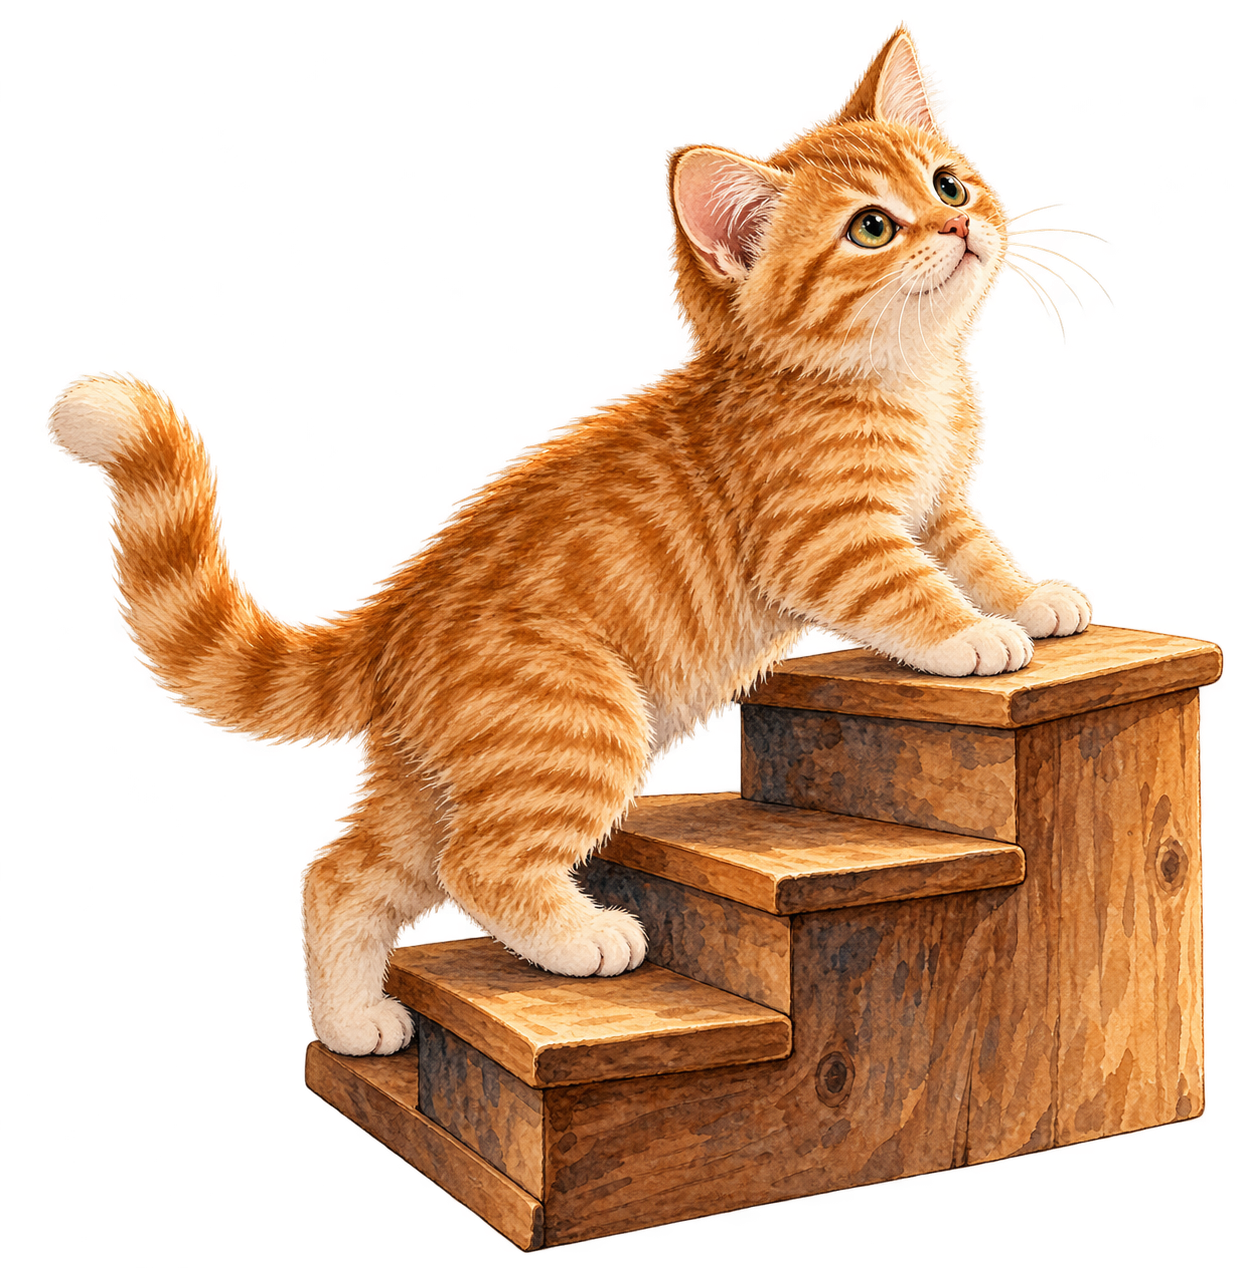
\includegraphics[width=54mm,height=58mm,keepaspectratio]{images/unique/art-13.png}
\end{wrapfigure}
\textit{Доказательство.} Запишем одну и ту же сумму в прямом и обратном порядке. При сложении получим \(2S_N=(a_1+a_N)+(a_2+a_{N-1})+\cdots+(a_N+a_1)\). В каждой из \(N\) скобок сумма равна \(2a_1+(N-1)d=a_1+a_N\). Деление на \(2\) даёт первую формулу, а подстановка общего члена — вторую. Рассуждение не зависит от чётности \(N\).\hfill\(\square\)
\par\WFclear\end{minipage}\end{lrbox}%
\ifdim\dimexpr\ht\CatFlowBox+\dp\CatFlowBox\relax<64mm\dp\CatFlowBox=\dimexpr64mm-\ht\CatFlowBox\relax\fi%
\noindent\usebox{\CatFlowBox}\par\addvspace{5pt}

\begin{definition}
\term{Геометрическая прогрессия} (geometric progression) в этом сборнике — последовательность, для которой \(a_{n+1}=q a_n\) при всех \(n\geq1\). Постоянное число \(q\) называют \term{знаменателем прогрессии} (common ratio). Такое определение включает \(q=0\): тогда последовательность имеет вид \(a_1,0,0,\ldots\).
\end{definition}
\begin{theorem}[Общий член геометрической прогрессии]
При \(q\neq0\)
\[
a_n=a_1q^{n-1},\qquad n\geq1.
\]
При \(q=0\) отдельно имеем \(a_n=0\) для \(n\geq2\); значение \(a_1\) задано начальным условием.
\end{theorem}
\begin{proof}
При \(q\neq0\) база \(n=1\) даёт \(a_1q^0=a_1\). Из формулы для \(k\) следует \(a_{k+1}=q a_k=q a_1q^{k-1}=a_1q^k\). При \(q=0\) сначала \(a_2=0\), затем каждый следующий член равен \(0\cdot0=0\). Такое отдельное рассмотрение позволяет не использовать неопределённую запись \(0^0\).
\end{proof}
\begin{theorem}[Сумма геометрической прогрессии]
При \(q\neq1\)
\[
S_N=\frac{a_1(1-q^N)}{1-q}.
\]
При \(q=1\) имеем \(S_N=Na_1\). Формула для \(q\neq1\) верна также при \(q=0\).
\end{theorem}
\begin{proof}
Из рекуррентного правила
\(qS_N=a_2+a_3+\cdots+a_{N+1}\). Вычитая это равенство из \(S_N=a_1+a_2+\cdots+a_N\), получаем \((1-q)S_N=a_1-a_{N+1}=a_1(1-q^N)\). При \(q\neq1\) делим на \(1-q\). При \(q=1\) все члены равны \(a_1\), поэтому сумма равна \(Na_1\).
\end{proof}
\subsection*{Предел, монотонность и ограниченность}
\begin{definition}
Число \(L\) — \term{предел последовательности} (limit of a sequence) \((b_N)\), если для любого \(\varepsilon>0\) существует натуральное \(N_0\), такое что при всех \(N\geq N_0\) выполнено \(|b_N-L|<\varepsilon\). Запись: \(\lim_{N\to\infty}b_N=L\). Иными словами, все достаточно поздние члены попадают в любой заранее выбранный интервал вокруг \(L\).
\end{definition}
\begin{definition}
Последовательность \((a_n)\) \term{не убывает} (is nondecreasing), если \(a_{n+1}\geq a_n\) для всех \(n\), и \term{не возрастает} (is nonincreasing), если \(a_{n+1}\leq a_n\). В обоих случаях её называют \term{монотонной} (monotone). Если неравенства строгие, говорят о строго возрастающей или строго убывающей последовательности.
\end{definition}
\begin{definition}
Последовательность \term{ограничена сверху} (bounded above), если существует число \(M\), такое что \(a_n\leq M\) при всех \(n\). Она \term{ограничена снизу} (bounded below), если существует \(m\) с \(m\leq a_n\) при всех \(n\). Если выполнены оба условия, последовательность \term{ограничена} (bounded).
\end{definition}
\begin{definition}
Число \(L\) называют \term{супремумом, или точной верхней гранью} (supremum, least upper bound) непустого множества \(A\subseteq\mathbb R\), если \(a\leq L\) для всех \(a\in A\), но никакое меньшее число не обладает этим свойством. Обозначение: \(L=\sup A\).
\end{definition}
\begin{definition}
Число \(m\) — \term{нижняя грань} (lower bound) множества \(A\subseteq\mathbb R\), если \(m\le a\) для каждого \(a\in A\).\end{definition}
\begin{definition}\term{Инфимум, или точная нижняя грань} (infimum; greatest lower bound) непустого множества — наибольшая его нижняя грань. Обозначение: \(\inf A\). Инфимум не обязан принадлежать самому множеству.
\end{definition}
Для \(A=(0;1]\) имеем \(\inf A=0\), \(\sup A=1\). Наименьшего элемента нет, а наибольший равен \(1\). Нельзя путать нижнюю грань с наименьшим элементом: граница описывает всё множество и может лежать вне него.
\begin{axiom}[Полнота действительных чисел]
\term{Аксиома полноты} (completeness axiom): каждое непустое множество действительных чисел, ограниченное сверху, имеет действительный супремум.
\end{axiom}
\begin{theorem}[Существование инфимума]
Всякое непустое ограниченное снизу множество \(A\subseteq\mathbb R\) имеет инфимум. Если \(-A=\{-a:a\in A\}\), то \(\inf A=-\sup(-A)\).
\end{theorem}
\begin{proof}
Множество \(-A\) непусто и ограничено сверху. Пусть \(L=\sup(-A)\), существующий по полноте. Из \(-a\le L\) получаем \(-L\le a\), так что \(-L\) — нижняя грань \(A\). Если \(b\) — любая нижняя грань, то \(-b\) — верхняя грань \(-A\), откуда \(L\le-b\), то есть \(b\le-L\). Следовательно, \(-L\) — наибольшая нижняя грань.
\end{proof}
\begin{theorem}[Сходимость монотонной ограниченной последовательности]
Всякая неубывающая и ограниченная сверху последовательность сходится. Её предел равен \(L=\sup\{a_n:n\in\mathbb N\}\). Всякая невозрастающая и ограниченная снизу последовательность также сходится. Следовательно, любая монотонная ограниченная последовательность имеет конечный предел.
\end{theorem}
\par\addvspace{5pt}\begin{lrbox}{\CatFlowBox}\begin{minipage}[t]{\linewidth}
\setlength{\parskip}{5pt}\setlength{\columnsep}{4.5mm}\setlength{\intextsep}{0pt}
\begin{wrapfigure}[12]{r}{54mm}
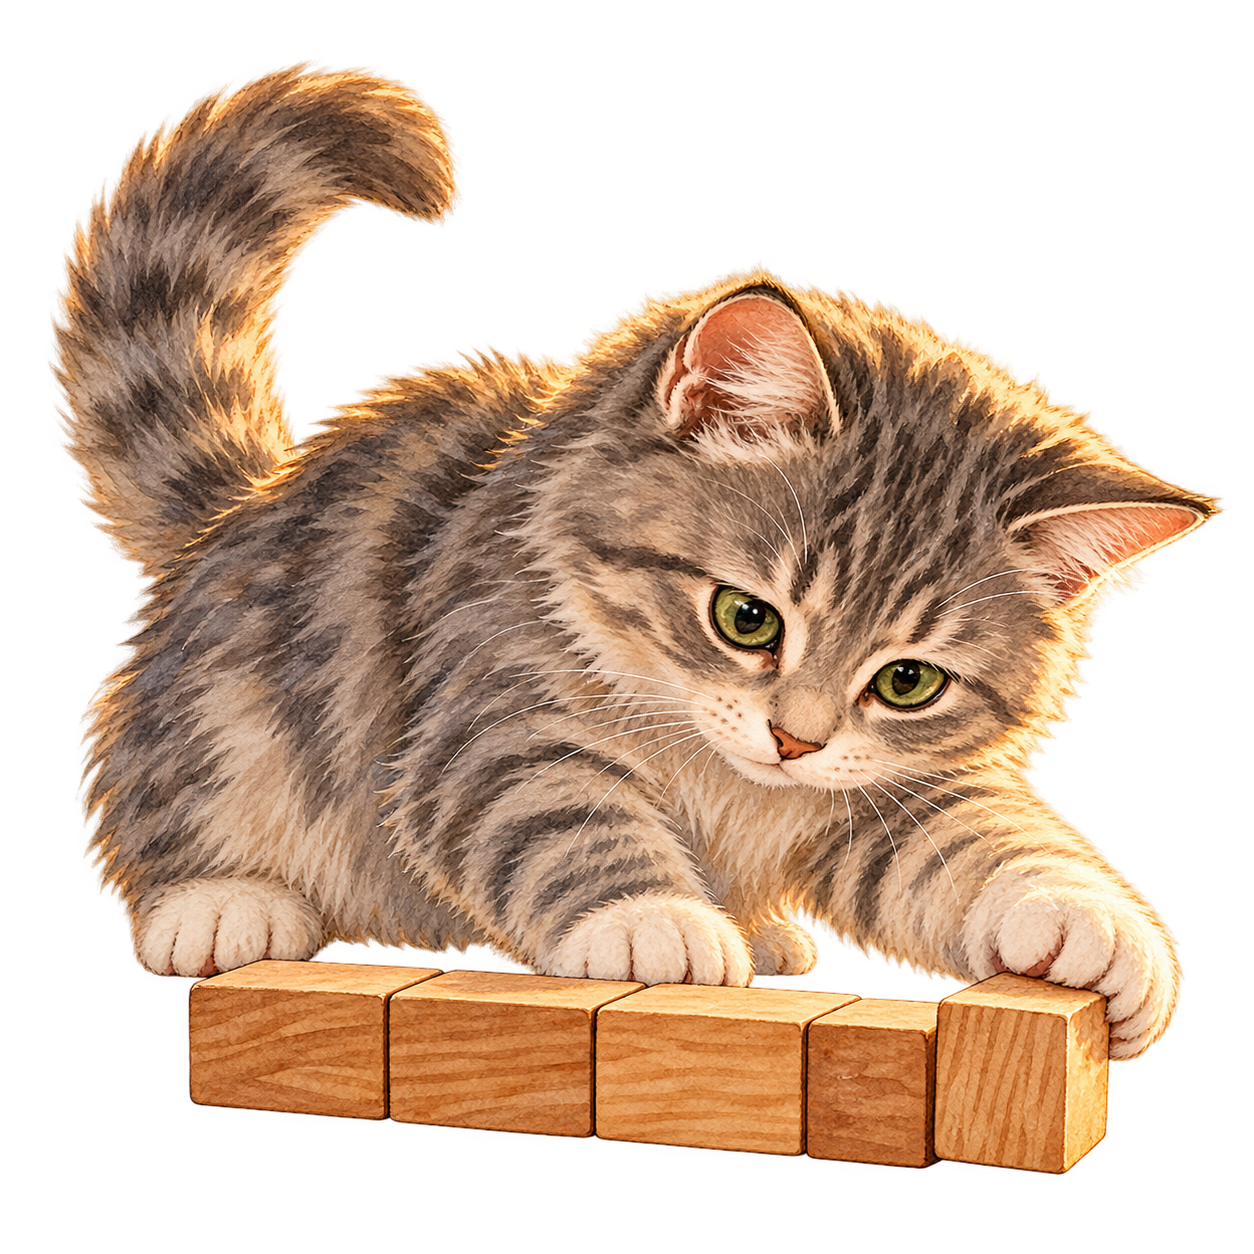
\includegraphics[width=54mm,height=58mm,keepaspectratio]{images/unique/art-20.png}
\end{wrapfigure}
\textit{Доказательство.} Для неубывающей последовательности супремум \(L\) существует по аксиоме полноты. Выберем любое \(\varepsilon>0\). Число \(L-\varepsilon\) не является верхней гранью, поэтому существует номер \(N\), для которого \(a_N>L-\varepsilon\). При всех \(n\geq N\) по монотонности \(a_n\geq a_N\), а по свойству верхней грани \(a_n\leq L\). Значит, \(L-\varepsilon<a_n\leq L\), то есть \(|a_n-L|<\varepsilon\). Это и означает \(a_n\to L\).

Для невозрастающей и ограниченной снизу последовательности \((a_n)\) последовательность \((-a_n)\) не убывает и ограничена сверху. Уже доказанный случай даёт \(-a_n\to B\), откуда \(a_n\to-B\), поскольку \(|a_n-(-B)|=|-a_n-B|\).\hfill\(\square\)
\par\WFclear\end{minipage}\end{lrbox}%
\ifdim\dimexpr\ht\CatFlowBox+\dp\CatFlowBox\relax<64mm\dp\CatFlowBox=\dimexpr64mm-\ht\CatFlowBox\relax\fi%
\noindent\usebox{\CatFlowBox}\par\addvspace{5pt}

Условие с \(\varepsilon\) придаёт словам «сколь угодно близко» точный смысл: сначала выбирается любая положительная точность \(\varepsilon\), и только после этого подбирается номер \(N\), начиная с которого \emph{все} члены удовлетворяют \(|a_n-L|<\varepsilon\). Единого заранее фиксированного \(N\) для всех точностей не требуется.

\subsection*{Бесконечная сумма}
\begin{definition}
\term{Бесконечный ряд} (infinite series) \(\sum_{n=1}^{\infty}a_n\) \term{сходится} (converges) к числу \(S\), если его частичные суммы \(S_N\) имеют предел \(S\). Число \(S\) называют \term{суммой ряда} (sum of a series). Если такого конечного предела нет, ряд \term{расходится} (diverges).
\end{definition}
\begin{theorem}[Бесконечная геометрическая сумма]
Пусть \(a_{n+1}=q a_n\). При \(|q|<1\)
\[
\sum_{n=1}^{\infty}a_n=\frac{a_1}{1-q}.
\]
Если \(a_1\neq0\), условие \(|q|<1\) также необходимо для сходимости. В частности, при \(q=1\) и при \(q=-1\) такой ряд расходится.
\end{theorem}
\begin{proof}
Сначала покажем \(q^N\to0\) при \(|q|<1\). Случай \(q=0\) непосредственен. Если \(0<r=|q|<1\), то \(r=\frac1{1+h}\) с \(h>0\). Неравенство \((1+h)^N\geq1+Nh\) доказывается индукцией: после умножения \(1+Nh\) на \(1+h\) получаем \(1+(N+1)h+Nh^2\geq1+(N+1)h\). Значит, \(|q^N|=r^N\leq\frac1{1+Nh}\), а эта верхняя граница становится меньше любого \(\varepsilon>0\) при достаточно большом \(N\).

По формуле конечной суммы
\[
\left|S_N-\frac{a_1}{1-q}\right|=\frac{|a_1|\,|q|^N}{|1-q|}\longrightarrow0.
\]
При \(a_1=0\) все суммы уже равны нулю. Если \(a_1\neq0\) и \(|q|\geq1\), то \(|a_n|=|a_1||q|^{n-1}\geq|a_1|\), поэтому \(a_n\) не стремится к нулю. Но из сходимости \(S_N\to S\) обязательно следует \(a_N=S_N-S_{N-1}\to0\): разность ограничена сверху величиной \(|S_N-S|+|S_{N-1}-S|\), и оба слагаемых стремятся к нулю. Получили противоречие.

Наглядно, при \(q=1\) суммы \(S_N=Na_1\) неограниченно растут по модулю. При \(q=-1\) они чередуются: \(S_{2k}=0\), \(S_{2k-1}=a_1\); при \(a_1\neq0\) единого предела нет.
\end{proof}
\begin{example}
\(1+\frac12+\frac14+\cdots=2\). При этом первые \(N\) слагаемых дают \(S_N=2(1-2^{-N})\), а недостающая до \(2\) величина равна \(2^{1-N}\) и стремится к нулю.
\end{example}

\Needspace{7\baselineskip}\section*{Задачи}
\begingroup\setlength{\parskip}{3pt}
\noindent\begin{minipage}[t]{\linewidth}\textbf{12.1.} Последовательность задана формулой \(a_n=3n-2\), \(n\geq1\). Выпишите первые пять членов и найдите \(a_{10}\).\par\end{minipage}\par
\noindent\begin{minipage}[t]{\linewidth}\textbf{12.2.} Для \(a_n=\dfrac{(-1)^n}{n}\) выпишите первые четыре члена. Укажите знак \(a_{25}\) и знак \(a_{26}\).\par\end{minipage}\par
\noindent\begin{minipage}[t]{\linewidth}\textbf{12.3.} Дано \(a_1=2\), \(a_{n+1}=2a_n-1\). Выпишите первые пять членов последовательности.\par\end{minipage}\par
\noindent\begin{minipage}[t]{\linewidth}\textbf{12.4.} Последовательность \(3,7,11,15,\ldots\) — арифметическая прогрессия. Найдите её разность и формулу общего члена.\par\end{minipage}\par
\noindent\begin{minipage}[t]{\linewidth}\textbf{12.5.} В арифметической прогрессии \(a_1=7\), \(d=-3\). Найдите \(a_8\).\par\end{minipage}\par
\noindent\begin{minipage}[t]{\linewidth}\textbf{12.6.} В арифметической прогрессии \(a_3=11\), \(a_9=35\). Найдите \(d\) и \(a_1\).\par\end{minipage}\par
\noindent\begin{minipage}[t]{\linewidth}\textbf{12.7.} Найдите сумму первых двадцати членов арифметической прогрессии с \(a_1=5\) и \(d=2\).\par\end{minipage}\par
\noindent\begin{minipage}[t]{\linewidth}\textbf{12.8.} Последовательность \(3,-6,12,-24,\ldots\) — геометрическая прогрессия. Найдите \(q\), формулу \(a_n\) и \(a_6\).\par\end{minipage}\par
\noindent\begin{minipage}[t]{\linewidth}\textbf{12.9.} В геометрической прогрессии \(a_1=81\), \(q=\dfrac13\). Найдите \(a_5\).\par\end{minipage}\par
\noindent\begin{minipage}[t]{\linewidth}\textbf{12.10.} В действительной геометрической прогрессии \(a_2=6\), \(a_5=48\). Найдите \(q\) и \(a_1\).\par\end{minipage}\par
\noindent\begin{minipage}[t]{\linewidth}\textbf{12.11.} Вычислите сумму \(1+2+4+\cdots+128\). Сначала определите число слагаемых.\par\end{minipage}\par
\noindent\begin{minipage}[t]{\linewidth}\textbf{12.12.} Найдите сумму бесконечного ряда \(18-6+2-\dfrac23+\cdots\). Объясните, почему геометрическая сумма здесь существует.\par\end{minipage}\par
\noindent\begin{minipage}[t]{\linewidth}\textbf{12.13.} В первую неделю в копилку положили \(100\) рублей, а в каждую следующую — на \(50\) рублей больше, чем в предыдущую. Сколько рублей положили за \(12\) недель?\par\end{minipage}\par
\noindent\begin{minipage}[t]{\linewidth}\textbf{12.14.} В первом ряду зала \(12\) мест, а в каждом следующем на \(2\) места больше. Всего \(20\) рядов. Найдите число мест в последнем ряду и во всём зале.\par\end{minipage}\par
\noindent\begin{minipage}[t]{\linewidth}\textbf{12.15.} В игре за первый день дают \(2\) монеты, а каждый следующий день награду удваивают. Найдите награду за седьмой день и общее число монет за первые семь дней.\par\end{minipage}\par
\par\addvspace{5pt}\begin{lrbox}{\CatFlowBox}\begin{minipage}[t]{\linewidth}
\setlength{\parskip}{5pt}\setlength{\columnsep}{4.5mm}\setlength{\intextsep}{0pt}
\begin{wrapfigure}[12]{l}{54mm}

\includegraphics[width=54mm,height=58mm,keepaspectratio]{images/unique/art-30.png}
\end{wrapfigure}
\textbf{12.16.} Докажите с помощью формулы суммы арифметической прогрессии, что \(1+3+5+\cdots+(2N-1)=N^2\) для любого натурального \(N\).\par

\textbf{12.17.} Докажите, что ряд \(a-a+a-a+\cdots\) не имеет суммы в смысле предела частичных сумм, если \(a\neq0\).\par

\textbf{12.18.}\starmark{} Дано \(a_1=3\), \(a_{n+1}=2a_n+1\). Найдите формулу общего члена и сумму первых десяти членов.\par

\textbf{12.19.}\starmark{} В арифметической прогрессии \(d>0\), \(a_2+a_5=34\), \(a_3a_4=280\). Найдите \(a_1\), \(d\) и \(S_{10}\).\par

\textbf{12.20.}\starmark{} Суммируют числа \(64,16,4,1,\ldots\). Найдите бесконечную сумму \(S\), формулу остатка \(R_N=S-S_N\) и наименьшее натуральное \(N\), при котором \(R_N<\dfrac1{10}\).\par

\textbf{12.21.} Для множества \((-2;5]\) найди супремум, инфимум, наибольший и наименьший элементы, если они существуют.\par

\textbf{12.22.} Найди точные грани множества \(A=\{1+\dfrac1n:n\in\mathbb N\}\). Принадлежат ли они \(A\)? Обоснуй ответ.\par

\textbf{12.23.} Для \(A=\{-3,2,7\}\) перечисли все нижние и верхние грани. Укажи точные грани.\par

\textbf{12.24.} Пусть непустое \(A\subseteq\mathbb R\) ограничено снизу, \(c\in\mathbb R\). Докажи \(\inf\{c+a:a\in A\}=c+\inf A\).\par
\par\WFclear\end{minipage}\end{lrbox}%
\ifdim\dimexpr\ht\CatFlowBox+\dp\CatFlowBox\relax<64mm\dp\CatFlowBox=\dimexpr64mm-\ht\CatFlowBox\relax\fi%
\noindent\usebox{\CatFlowBox}\par\addvspace{5pt}

\endgroup
